\chapter{Build C/C++ code}

\section{compile code} 
% using g++/clang

\subsection{build steps} 

\texttt{gcc HelloWorld.c}  compiles and links source file HelloWorld.c into executable a.out


\texttt{gcc -o HelloWorld HelloWorld.c} : Compile and link source file HelloWorld.c into executable HelloWorld. \texttt{-o}: specifies the output executable filename (HelloWorld)


To run \texttt{./a.out}: (./ - include current path, by default current directory is not included)


\texttt{g++ -o HelloWorld HelloWorld.cpp} : 


\texttt{g++ -c HelloWorld.c} : Compile only with option -c, output is Helloworld.o


Preprocessor talking with compiler directly 


\subsubsection{Overview of compilation process}%
\label{ssub:overview_of_compilation_process}
GCC compiles a C/C++ program into executable in four steps as shown in the below diagram.  For example, a "gcc -o hello.exe hello.c" is carried out as follows:

\begin{enumerate}
  \item Pre-processing: via the GNU C Preprocessor (cpp.exe), which includes the headers (\#include) and expands the macros (\#define). 
  \item Compilation: The compiler compiles the pre-processed source code into assembly code for a specific processor. 
  \item Assembly: The assembler (as.exe) converts the assembly code into machine code in the object file "HelloWorld.o". 
  \item Linker: Finally, the linker (ld.exe) links the object code with the library code to produce an executable file "HelloWorld". 
\end{enumerate}

\label{sec:figures}
\begin{figure}[h]
\caption{Compilation steps}
\centering
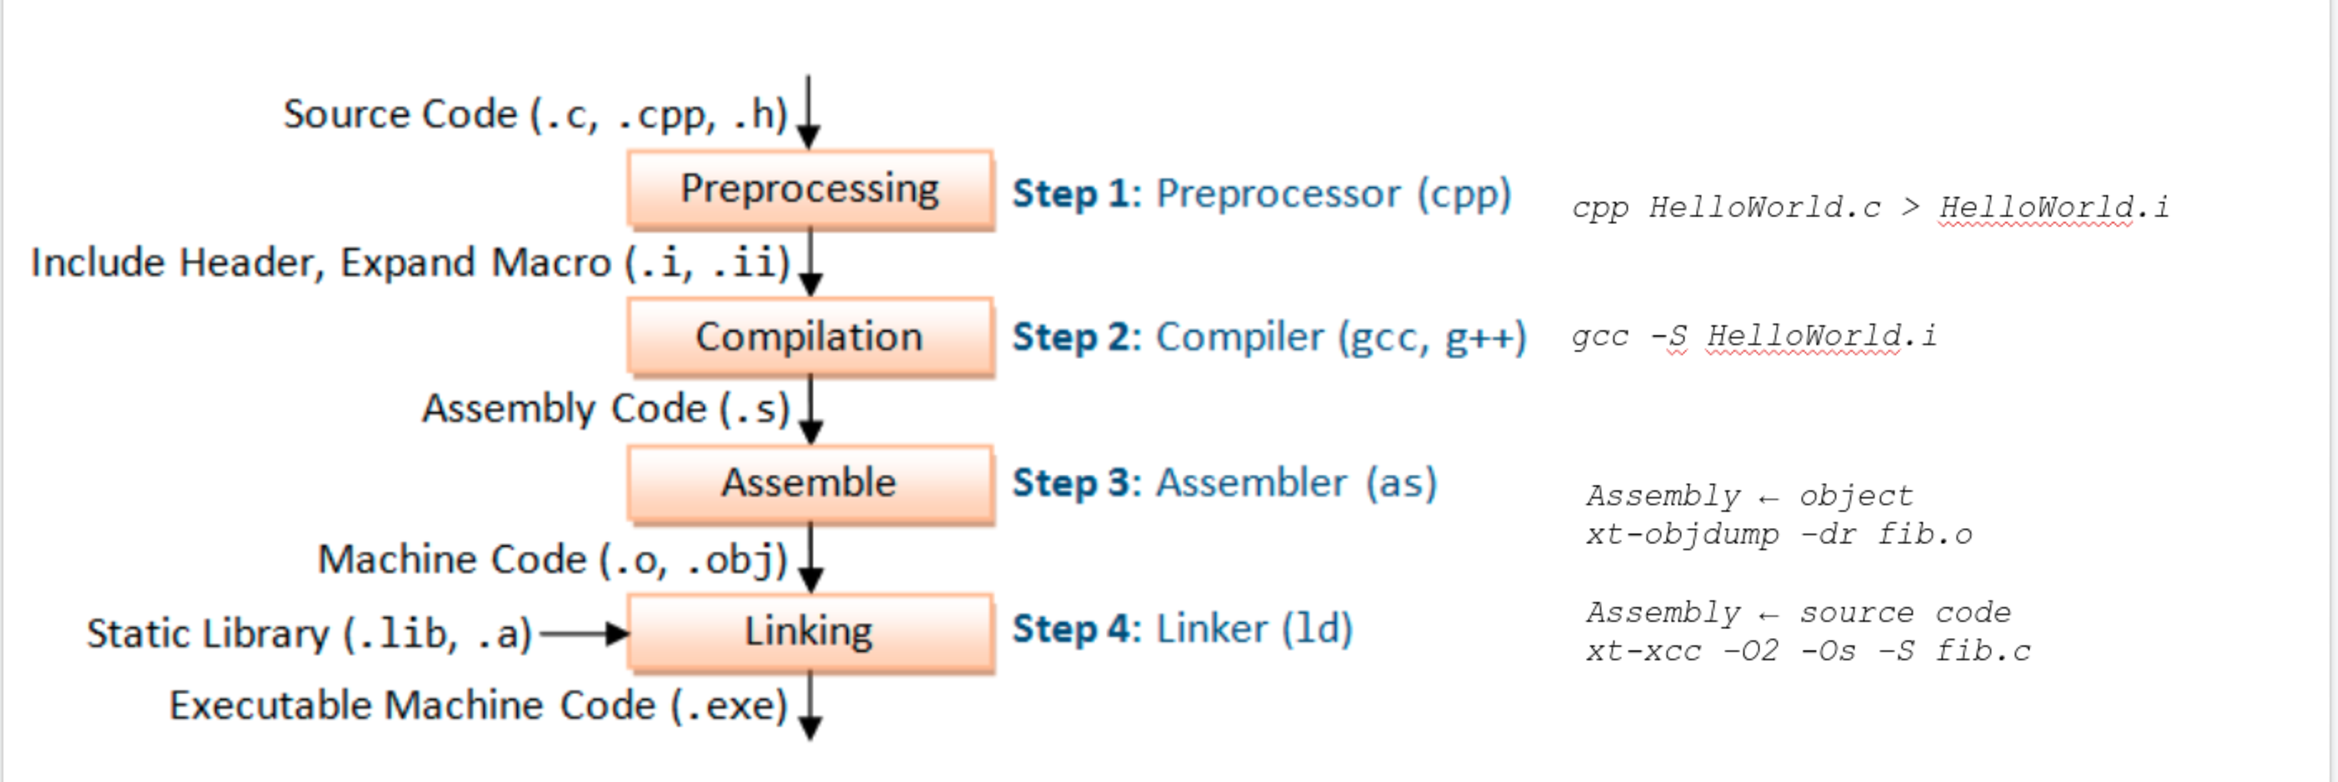
\includegraphics[width=0.5\textwidth]{./build/compilation_steps.pdf}
\end{figure}


\section{Libraries} 
%locations
%LD_LIBRARY
%ldd command

\subsubsection*{Creating Libraries using ar command}%
\label{ssub:creating_libraries_using_ar_command}
ar is an archive tool used to combine objects to create an archive file with .a extension, also known as library.

\href{https://www.thegeekstuff.com/2010/08/ar-command-examples/}{UNIX ar Examples: How To Create, View, Extract, Modify C Archive Files} 

\subsection{pthread} 
% TODO [vikki @22/08/23]: add an examplw with pthread library. %

\subsection{Makefile} 

A \texttt{make} determines which pieces of a large program need to be recompiled, and issues the commands to recompile them.

You can use \texttt{make} with any programming language whose compiler can be run with a shell command. Indeed, \texttt{make} is not limited to programs. You can use it to describe any task where some files must be updated automatically from others whenever the others change.
For example, I implemented genome processing pipelines using \texttt{make}.

The \texttt{make} program uses the \texttt{make} data base and the last-modification times of the files to decide which of the files need to be updated.




\subsubsection{Getting help}%
\label{ssub:getting_help}
\begin{itemize}
  \item \texttt{man make}
  \item \texttt{make --help}
  \item \href{https://www3.ntu.edu.sg/home/ehchua/programming/cpp/gcc_make.html} { GCC and Make Compiling, Linking and Building C/C++ Applications }
    \item \href{Managing Projects with GNU Make, Third Edition}{https://www.oreilly.com/openbook/make3/book/} 
    \item \href{https://www.gnu.org/software/make/manual/make.html\#toc-Overview-of-make} {GNU make}
\end{itemize}


\subsubsection{Makefile}%
A \texttt{make} recognizes \texttt{makefile}, \texttt{Makefile} and \texttt{GNUMakefile}. But if the name is different you can run \texttt{make -f make\_file\_name}.

A \texttt{makefile} consists of a set of rules. A rule consists of three parts: targets, a list of prerequisites (dependents) and commands, as follow,

\begin{listing}[!ht]
\usemintedstyle{vim}
\begin{minted}[linenos]{bash}
  target1 target2 : prerequisite1 prerequisite2
    command1
    command2
\end{minted}
\caption{makefile rules}
\label{makefile_rules}
\end{listing}

Comments start with character `\#' and last until end of the line.
\textbf{`\#' does not introduce comment in the text of commands. The entire line, including the `\#' and subsequent characters, is passed to the shell for execution.}


Long line can be broken and continued in several lines via a back-slash (\textbackslash).


The target and prerequisites are separated by a colon (:). The command must be preceded by a \textbf{tab (NOT spaces)}.

A target is usually the name of a file that is generated by a program.
A target can also be the name of an action to carry out, such as \texttt{clean}.

A prerequisite is a file that is used as input to create the target.
A target often depends on several files.

The prerequisites must exist before the target can be successfully created.

The commands are those shell commands that create the target from the prerequisites.

When \texttt{make} evaluates a rule, it begins by finding the files in the prerequisites.
If any of the prerequisites has an associated rule, \texttt{make} attempts to update those first.
More importantly, if the target is newer than prerequisites, the command will not be run.

If a target is included as a command-line argument, that target is updated.
If no command-line targets are given, then the first target in the file is used, called the default goal.

A recipe is an action that \texttt{make} carries out. A recipe may have more than one command, either on the same line or each on its own line.

\subsubsection{Rules}%
\label{ssub:rules}

\begin{enumerate}
  \item \textbf{Explicit rules} indicate a specific target to be updated if it is out of date with respect to any of its prerequisites.
  \item \textbf{Implicit rules} are either pattern rules or suffix rules found in the rules database built-in to make.
    It is not necessary to spell out the recipes for compiling the individual C source files, because make can figure them out: it has an implicit rule for updating a ‘.o’ file from a correspondingly named ‘.c’ file using a ‘cc -c’ command. For example, it will use the recipe ‘cc -c main.c -o main.o’ to compile main.c into main.o. We can therefore omit the recipes from the rules for the object files.
  \item \textbf{Pattern rules} use wild cards instead of explicit filenames. This allows make to apply the rule any time a target file matching the pattern needs to updated.  These conventions allow make to simplify rule creation by recognizing common filename patterns and providing built-in rules for processing them. When make searches for a pattern rule to apply, it first looks for a matching pattern rule target. Next make looks at the prerequisites of the pattern rule by substituting the stem into the prerequisite pattern
  \item \textbf{Static pattern} rules are like regular pattern rules except they apply only to a specific list of target files
\end{enumerate}

\subsubsection{Explicit Rules}%
\label{ssub:explicit_rules}

In the “forward” direction the rule says that if the lexer.c has been updated, perform the action to update vpath.o.

In the “backward” direction, the rule says that if we need to make or use vpath.o ensure that lexer.c is up to date first

\begin{listing}[!ht]
\usemintedstyle{vim}
\begin{minted}[linenos]{bash}
  vpath.o: lexer.c
\end{minted}
\caption{Forward and bacward dependecy}
\label{makefile_bi_directional_dependency}
\end{listing}

If a target has already been seen and exists in the graph, any additional prerequisites are appended to the target file entry in make’s dependency graph.


\begin{listing}[!ht]
\usemintedstyle{vim}
\begin{minted}[linenos]{bash}
  vpath.o: vpath.c make.h config.h getopt.h gettext.h dep.h
  vpath.o: filedef.h hash.h job.h commands.h variable.h vpath.h
\end{minted}
\caption{Append rules}
\label{makefile_append_rules}
\end{listing}

A rule can have more than one target. This means that each target has the same set of prerequisites as the others. If the targets are out of date, the same set of actions will be performed to update each one.


\begin{listing}[!ht]
\usemintedstyle{vim}
\begin{minted}[linenos]{bash}
  vpath.o variable.o: make.h config.h getopt.h gettext.h dep.h
  ==
  vpath.o: make.h config.h getopt.h gettext.h dep.h
  variable.o: make.h config.h getopt.h gettext.h dep.h
\end{minted}
\caption{Explicit rules}
\label{makefile_explicit_rules}
\end{listing}

Each target may have different commands. For example,

\begin{listing}[!ht]
\usemintedstyle{vim}
\begin{minted}[linenos]{bash}
  vpath.o: vpath.c make.c
  vpath.o: vpath.c
    $(COMPILE.c) $(RULE_FLAGS) $(OUTPUT_OPTION) $<

  vpath.o: make.c
    $(COMPILE.c) $(RULE_FLAGS2) $(OUTPUT_OPTION) $<
\end{minted}
\caption{Different command}
\label{different_command}
\end{listing}

\subsubsection{Wildcards}%
\label{ssub:make_wildcards}

\texttt{make}’s wildcards are identical to the Bourne shell’s: `$\sim$', `*', `?', ``[...]'', and ``[\^{}...]''

``.*'' expands to all the files containing a period.

`?' represents any single character,

``[...]'' represents a character class.

To negate character class use ``[\^{}...]''

`$\sim$' character can be used to represent the current user’s home directory


\subsubsection{Phony / Artificial Targets }%
\label{ssub:make_phony}

A target that does not represent a file is called a phony target.(ex clean, install and all).
phony targets will always be executed.
To avoid this problem, GNU make includes a special target, \texttt{.PHONY}, to tell make that a target is not a real file.


\texttt{.PHONY} tells make that this file does not follow the normal rules for making a target file from a source file
The output of make can be made much easier to read if major targets are commented in the make output. Phony targets are a useful way to accomplish this.


\subsubsection{Empty Targets }%
\label{ssub:make_empty}
 But suppose we have some command, with no output file, that needs to be performed only occasionally and we don’t want our dependents updated?

\subsubsection{ Finding Files with VPATH and vpath }%
\label{ssub:make_vpth}

The \texttt{VPATH} variable consists of a list of directories to search when make needs a file.
The list will be searched for targets as well as prerequisites.
but not for files mentioned in command scripts ( direct file names does not work, variable works).
make will search each directory for any file it needs. If a file of the same name exists in multiple places in the \texttt{VPATH} list, make grabs the first one. Sometimes this can be a problem.
The \texttt{vpath} directive is a more precise way to achieve our goals


\subsubsection{Variables}%
\label{ssub:make_variables}

The simplest ones have the syntax: \$(variable-name).
Variables can contain almost any text, and variable names can contain most characters including punctuation.
The only characters actually disallowed in a variable name are :, \#, and =
Variables are case-sensitive.
A variable begins with a \$ and is enclosed within parentheses (...) or braces \{...\}, for example, \$(CC) and \$\{CC\_FLAGS\}.
Single character variables do not need the parentheses, for example \$@ and \$\^{}
Two types of variables in make: simply expanded variables and recursively expanded variables.

Automatic Variables

Automatic variables are set by make after a rule is matched.
There are six \textbf{core} automatic variables:

\begin{enumerate}
  \item \$\%: The filename element of an archive member specification
  \item \$@: The target filename
  \item \$*: The target filename without extension.
  \item \$+: All the prerequisites
  \item \$\^{}: All the prerequisites, but discard duplicates
  \item \$$\langle$: The first prerequisite
  \item \$?: prerequisites, newer than the target
\end{enumerate}

Variables Assignments

There are four types of assignments
\begin{enumerate}
  \item :=  simply expanded variables - its right-hand side is expanded immediately upon reading the line from the makefile (same as most programming and scripting languages)
  \item = recursively expanded variable- its right-hand side is simply slurped up by make and stored as the value of the variable without evaluating or expanding it in any way. Instead, the expansion is performed when the variable is used.
  \item ?= conditional variable assignment operator.This operator will perform the requested variable assignment only if the variable does not yet have a value.
  \item += append variable assignment operator. Appending the supplied value to the existing value (or setting to that value if the variable didn't exist)
\end{enumerate}

macro to combine may command together


When Variables Are Expanded

make performs its job in two phases

\begin{enumerate}
  \item first phase, make reads the makefile and any included makefiles. At this time, variables and rules are loaded into make's internal database and the dependency graph is created.
  \item second phase, make analyzes the dependency graph and determines the targets that need to be updated, then executes command scripts to perform the required updates
\end{enumerate}
For variable assignments, the left-hand side of the assignment is always expanded immediately when make reads the line during its first phase
The right-hand side of = and ?= are deferred until they are used in the second phase
The right-hand side of := is expanded immediately
The right-hand side of += is expanded immediately if the left-hand side was originally defined as a simple variable. Otherwise, its evaluation is deferred
For macro definitions (those using define), the macro variable name is immediately expanded and the body of the macro is deferred until used
For rules, the targets and prerequisites are always immediately expanded while the commands are always deferred


Target- and Pattern-Specific Variables

Wanted to redefine a variable for just a single rule or pattern. But that should not be provided to other compiles
These are variable definitions attached to a target that are valid only during the processing of that target and any of its prerequisites
When the gui.o target is finished, CPPFLAGS will revert to its original value.

Where Variables Come From
\begin{enumerate}[(i)]
  \item file
  \item command line
  \item environment
  \item automatic
\end{enumerate}

\subsection{bazel}
